\documentclass[lettersize,journal]{IEEEtran}
% =====================================================================
%  IEEEtran 主文件说明（写给未来的你/合作者看的注释）
% =====================================================================
% 1) 文件结构（推荐的组织方式）
%    - 本文件：KAMMT-trans.tex（主入口，负责：导言区、标题作者信息、整体排版、文末参考文献）
%    - 图像文件：建议统一放到 Figures/ 目录下，例如：Figures/xxx.pdf / .png / .jpg
%    - 参考文献库：references.bib（BibTeX 数据库，文末通过 \bibliography{references.bib} 调用）
%    - 如果正文很长：可把各章节拆到子文件（例如 sections/intro.tex），再在主文件用
%      \input{sections/intro} 或 \include{sections/intro} 组织。
%
% 2) 编译方式（Overleaf）
%    - Overleaf 一般会自动运行（pdfLaTeX + BibTeX + pdfLaTeX + pdfLaTeX）来生成参考文献。
%    - 若你发现引用显示为 [?]：通常是 .bib 没编译成功或 key 不匹配。
%
% 3) 插入图片（graphicx）
%    - 单栏图（IEEE 常用）：
%        \begin{figure}[!t]
%          \centering
%          \includegraphics[width=\linewidth]{Figures/your-figure}
%          \caption{...}
%          \label{fig:your_label}
%        \end{figure}
%      说明：文件扩展名可省略（如 your-figure.png/pdf），LaTeX 会自动选择。
%
%    - 跨双栏大图：用 figure* 环境（你在文中已用到）：
%        \begin{figure*}[!t] ... \end{figure*}
%
%    - 子图（subfig）：
%        \subfloat[子图1]{\includegraphics[width=0.48\linewidth]{Figures/a}}
%        \subfloat[子图2]{\includegraphics[width=0.48\linewidth]{Figures/b}}
%
%    - 图的引用：
%        \ref{fig:your_label} 或（已加载 cleveref）\cref{fig:your_label}
%
% 4) 引用文献（cite + BibTeX）
%    - 文中引用：\cite{key}；多个条目：\cite{key1,key2,key3}
%    - 在 references.bib 里新增/修改条目，确保条目的 key 与 \cite{} 一致。
%    - 文末参考文献：
%        \bibliographystyle{...}
%        \bibliography{references.bib}
%      说明：IEEE 期刊/会议通常使用 IEEEtran 的 bst（例如 IEEEtran/IEEEtranN），
%      你当前用的是 unsrt；如需严格 IEEE 样式，可改为：\bibliographystyle{IEEEtran}
%
% 5) 交叉引用（建议习惯）
%    - 公式：\label{eq:xxx}，文中 \cref{eq:xxx}
%    - 表格：\label{tab:xxx}，文中 \cref{tab:xxx}
%    - 小技巧：label 前缀统一（fig:/tab:/eq:/sec:）能极大降低维护成本。
% =====================================================================

\usepackage{amsmath,amssymb,amsfonts}
\usepackage{array}
\usepackage{booktabs}
\usepackage{multirow}

\usepackage{algorithm}
\usepackage{algorithmic}

\usepackage{graphicx}
\usepackage[cmyk]{xcolor}
\usepackage{textcomp}
\usepackage{soul}

% IEEE recommended sub-figures (use \subfloat, not subfigure environment)
\usepackage[caption=false,font=normalsize,labelfont=sf,textfont=sf]{subfig}

\usepackage{url}
\usepackage{verbatim}
\usepackage{cite}
\usepackage{stfloats}

% CJK + hyperlinks/cleveref (order matters: hyperref -> cleveref)
\usepackage{xeCJK}
\usepackage{hyperref}
\usepackage{cleveref}


\hyphenation{op-tical net-works semi-conduc-tor IEEE-Xplore}
% updated with editorial comments 8/9/2021

\begin{document}

\title{KAMT: Clinical Knowledge guided multi-modal learning based diagnosis of neurological disorders}
%知识增强型KAMT (Knowledge-Augmented multi-modal Transfomer)
%知识赋能型KEMT (Knowledge-Empowered Multi-Modal Transformer)
%知识引导协同多模态神经网络KG-SMMT (Knowledge-Guided Synergistic Multi-Modal Transformer)
%知识prompt提示词神经网络KPMT (Knowledge-Prompted Multi-Modal Transformer)
%知识注入型KIMT (Knowledge-Infused Multi-Modal Transformer)


\author{IEEE Publication Technology,~\IEEEmembership{Staff,~IEEE,}
        
}

% The paper headers
\markboth{Trans}%
{Author \MakeLowercase{\textit{et al.}}: KAMT}



\maketitle

\begin{abstract}
        euroimage samples and clinical metadata have been employed to conduct precision diagnosis for AD-related dementia(ADRD) and cognitive impairment.
        For precision diagnosis of neurodegenration, artificial intelligence approaches tend to rely heavily on sample size and data quality.
        To alleviate this over-reliance problem, dementia-specific knowledge played an essential role in enhancing the credibility and reliability of disease diagnostic methods. For the textual modality associated with AD and dementia, the semantic relations between biomedical entities were extracted and applied as domain knowledge to guide the learning of deep neural networks. Under the MML framework, this work proposes the KAMT architecture to enhance predictive accuracy and credibility in the diagnosis of neurological disorders.   
        
\end{abstract}

\begin{IEEEkeywords}
	Clinical knowledge, multi-omics integration, brain disease diagnosis.
\end{IEEEkeywords}

\section{Introduction}
\label{sec:introduction}

    \hl{Two essential points should be referred in this section. The first is the uniqueness of the extracted DemRKG, with comparison with common knowledge representations. Another perspective of KAMT is the knowledge-guided learning scheme. Soft embedding of DemRKG may be more suitable for established hard-concat way.}
    
    \IEEEPARstart{A}{ssessment} of brain diseases has become an important topic in precision medicine. For neurodegenerative diseases such as Parkinson's disease (PD) and Alzheimer's disease (AD), multimodal deep learning integrating diverse features has gradually become the mainstream approach in this field \cite{qiu2022multimodal,zhang2026multimodalpd}. Recent advanced frameworks have even attempted to ground diagnostic decisions in localized anatomy and clinical variables to improve transparency \cite{lin2025adlip,wood2026align}. Specifically, practical diagnostic pipelines typically involve extracting baseline information from Electronic Health Records (EHR)\cite{rajkomar2018scalable}, tracking the dynamic changes of clinical scales within Biomarkers (BM)\cite{marek2011parkinson}, and utilizing 3D-CNNs \cite{basaia2019automated} to preprocess MRI samples for capturing localized microstructural changes.

    However, lacking prior guidance on underlying pathological mechanisms, purely data-driven models heavily rely on isolated numerical computations and image feature extraction. By ignoring the critical semantic associations between biomedical entities in medical records, these approaches suffer from severe overfitting and performance degradation\cite{lu2021knowledge} when applied to multi-center clinical cohorts with heterogeneous feature distributions.

    
    With ADRD-specific knowledge representations, the Knowledge-Augmented learning scheme could provide a way to improve the model performance as well as reliability. It is noted that the quality of knowledge representations determines the prediction accuracy and model generalization ability in precision medicine \cite{chandak2023building}. Motivated by established works about large-scale biomedical knowledge graphs including SPOKE \cite{morris2023spoke} and PharmKG \cite{zheng2021pharmkg}, this work develops the dementia-specific knowledge graphs by extracting complicated causal relations between biomedical ontology that are associated with brain disease and cognitive decline.
    \hl{Which external biomedical knowledge was used in this study? How to corporate existing DemRKG and SPOKE/PharmKG?}
    
    Knowledge-augmented neural network learning architecture is another essential perspective in obtaining reliable predictions from multi-omics data. With external biomedical knowledge, relational knowledge graph named DemRKG has been constructed to capture causal relations for biomedical entities that are associated with dementia and cognitive decline. For neurological disorders, essential ontologies such as vascular dynamics and immune regulation have been encoded in the triplets in large-scale biomedical KG \cite{zhao2026kgt,sim2024gtad}. \textcolor{blue}{The contributions of the KAMT method were summarized as follows:}
    
\begin{itemize}
    \item Compact knowledge representations with high information density have been extracted and exploited in disease prediction;
    \item Clinical knowledge-augmented learning scheme has been proposed to integrate augmented knowledge representations and multi-modal learning;
    \item  For dementia and cognitive impairment, clinic knowledge has been extracted as triplets and incorporated into multimodal learning network;
    \item External knowledge source was introduced to obtain high-quality domain knowledge in the diagnosis of ADRD, with the proposed X-KD strategy.
    
    \cite{yang2015embedding}.
\end{itemize}

    \textcolor{blue}{Compact DemRKG play the role of high-quality clinical knowledge representations that are informative.}



\section{Related Works}

\subsection{Multimodal Deep Learning for the Diagnosis of Neurodegenerative Diseases}

Multimodal deep learning has become a mainstream paradigm for assessing Alzheimer's disease (AD) and related dementias. Many studies jointly model textual clinical records and imaging phenotypes to represent patients' complex pathological states \cite{jin2026multimodal}. Early approaches often relied on convolutional or recurrent architectures, while recent multimodal fusion models increasingly adopt attention-based designs. Although purely data-driven methods can achieve strong performance on curated benchmarks, they frequently suffer from distribution shift, overfitting, and degraded generalization when evaluated across sites or cohorts with heterogeneous acquisition protocols and feature distributions \cite{abugabah2025intelligent}. Moreover, due to the lack of explicit prior knowledge of disease mechanisms, these models may overemphasize surface correlations within modalities while neglecting clinically meaningful semantic connections between entities in medical narratives and cognitive scale outcomes.

\subsection{Biomedical Knowledge Graphs and Their Constraints in Clinical Tasks}

To alleviate the generalization bottleneck of data-driven multimodal approaches, integrating biomedical knowledge graphs (KGs) is considered a promising direction. Nevertheless, simply attaching large, general external knowledge graphs to the diagnostic workflow can introduce significant biological noise and dilute task-relevant signals. Conversely, lightweight domain-specific graphs built from local clinical records may be more aligned with downstream objectives but often lack the breadth of biomedical ontology and generalization capabilities. These limitations have prompted the development of task-adaptive relational diagnostic knowledge graphs to balance domain specificity and external ontology coverage.

\subsection{Knowledge-Guided Multimodal Fusion Frameworks}

    Established knowledge-guided neural networks generally operate in a shallow fusion regime: KG-derived node embeddings are treated as independent vectors and concatenated (or otherwise hard-connected) with image/text features near the network output \cite{chen2023knowledge}. Such designs implicitly equate discrete knowledge spaces with continuous representation spaces, limiting the extent to which domain knowledge can influence intermediate feature learning and cross-modal alignment. To obtain discriminative, fine-grained fusion, recent multimodal diagnostic models increasingly adopt Transformer-style self-/cross-attention to adaptively weight and align heterogeneous representations \cite{vaswani2017attention,kyritsis2025transformerfusionad,li2024hammf,du2025vitadreview,chen2026federatedvitad}. Building upon this, we designed knowledge-augmented  features in the cross-self-attention module, allowing knowledge to act as an implicit constraint, actively guiding and regulating multimodal feature learning.
    

    
\section{\textcolor{blue}{Clinically Guided Knowledge Augmentation with KAMT}}

    In precision diagnosis of brain diseases, knowledge graph embedding (KGE) methods aim to encode biomedical entities and their relations into a low-dimensional semantic space.
    Specifically, the KGE method learns low-rank entity representations by scoring observed triplets higher than corrupted ones. Representative models include TransE\cite{bordes2013translating}, DistMult, ComplEx\cite{trouillon2016complex}, and RotatE\cite{sun2019rotate}.

    \textcolor{blue}{We propose} a controlled relation graph refinement paradigm: task-specific multimodal seeds have been extracted and topological refinement has been conducted to build a dementia-oriented relational KG (DemRKG), \textcolor{blue}{which provides entity representations for downstream KAMT.}

\textcolor{blue}{The construction and representation-learning pipeline of DemRKG is illustrated in \cref{fig:dementia_hkg_flow}.}

\begin{figure*}[!t]
    \centering
    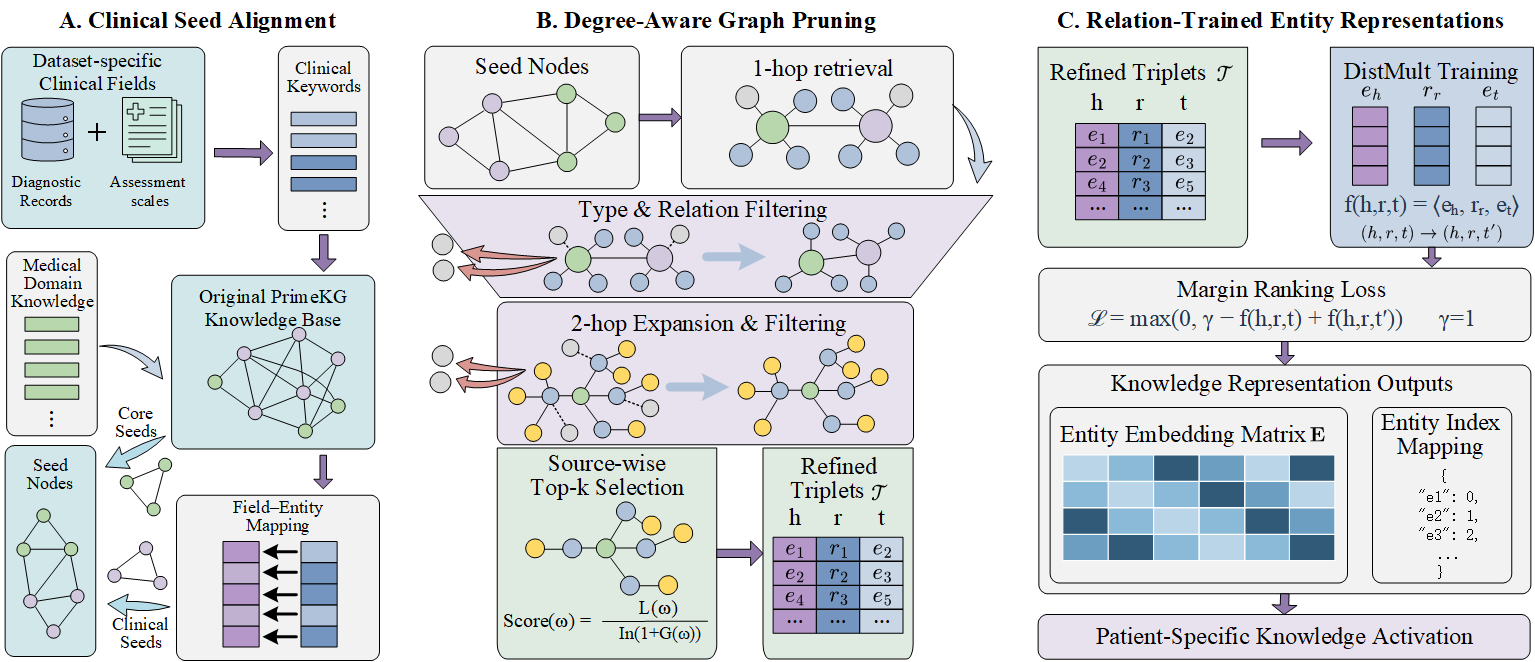
\includegraphics[width=\textwidth]{Figures/DemRKG流程图-EN.png}
    \caption{\textcolor{blue}{Construction and representation learning of DemRKG. (A) Clinical seed alignment with PrimeKG. (B) Degree-aware graph pruning: filtered one-hop edges are retained and merged with source-wise top-$k$ two-hop candidate edge records, followed by deduplication to form the refined triplets. (C) DistMult training produces relation-trained entity embeddings and an entity index mapping.}}
    \label{fig:dementia_hkg_flow}
\end{figure*}

\subsection{\textcolor{blue}{Refinement of DemRKG}}

\subsubsection{\textcolor{blue}{Clinical Seed Alignment}}

     \textcolor{blue}{Medical keywords are manually selected to reflect the diagnostic meaning of each dataset's clinical fields. Searches within the relevant entity types in PrimeKG $\mathcal{G}_0=(\mathcal{V}_0,\mathcal{R}_0,\mathcal{T}_0)$ return candidate entities, whose names are presented from shortest to longest for manual review. Selected standard entity names are entered into a dataset-specific field--entity dictionary and checked against PrimeKG. The validated pairs define $M:\mathcal{F}\rightarrow\mathcal{V}_0$, where $\mathcal{F}$ contains the matched clinical fields; their entities form $\mathcal{S}_{\mathrm{clinical}}$. In parallel, dataset-specific disease and molecular core candidates are manually selected based on medical domain knowledge, and those found in PrimeKG are retained as $\mathcal{S}_{\mathrm{core}}$. The resulting dataset-level seed set is}
     \begin{equation}
     \mathcal{S}
     =
     \mathcal{S}_{\mathrm{clinical}}
     \cup
     \mathcal{S}_{\mathrm{core}}.
     \label{eq:seed_set}
     \end{equation}

\subsubsection{\textcolor{blue}{Degree-Aware Graph Pruning}}

    \textcolor{blue}{One-hop edges are retrieved from the seed set $\mathcal{S}$. Let $\mathcal{B}_{\mathrm{type}}$ and $\mathcal{B}_{\mathrm{rel}}$ denote the blacklisted entity types and relations. For an edge set $\mathcal{U}\subseteq\mathcal{T}_0$, we remove edges with a blacklisted endpoint type or relation:}
    \begin{equation}
        {\color{blue}
        \begin{aligned}
        \mathcal{U}_{\mathrm{clean}}=\mathcal{U}\setminus\{(h,r,t)\in\mathcal{U}:\;&
        \operatorname{type}(h)\in\mathcal{B}_{\mathrm{type}}\\
        &\lor\operatorname{type}(t)\in\mathcal{B}_{\mathrm{type}}\\
        &\lor r\in\mathcal{B}_{\mathrm{rel}}\}.
        \end{aligned}
        }
        \label{eq:blacklist_filter}
    \end{equation}
    \textcolor{blue}{The blacklist filter is first applied to the one-hop edges. We expand the retained neighborhood to obtain candidate two-hop edges and filter these candidates in the same way. During two-hop expansion, protein--protein interaction (PPI) edges link proteins in the retained seed neighborhood to their interacting partners} \cite{barabasi2011network,cheng2019network}. \textcolor{blue}{To reduce the influence of highly connected nodes in the expanded graph, we define the following specificity score:}

    \begin{equation}
        Score(w) = \frac{L(w)}{\ln(1 + G(w))}
        \label{eq:spec-score}
    \end{equation}
    where \textcolor{blue}{$L(w)$ counts distinct candidate source nodes connected to $w$}, and \textcolor{blue}{$G(w)$ counts records in which $w$ occurs at either endpoint in PrimeKG}. \textcolor{blue}{The numerator measures a candidate target's connectivity to multiple sources, while the denominator penalizes its global degree. For each source, we select the top-$k$ candidate edge records according to their target-node scores. We then merge the selected records with the filtered one-hop edges and remove duplicate records to obtain the refined triplets $\mathcal{T}$.}

\subsubsection{\textcolor{blue}{Relation-Trained Entity Representations}}

    \textcolor{blue}{KG embeddings in $\mathbb{R}^d$ are pre-trained on the refined DemRKG triplets $\mathcal{T}$. DistMult scores each triplet as $f(h,r,t)=\langle\mathbf e_h,\mathbf r_r,\mathbf e_t\rangle$, and negative samples are generated by replacing tail entities. Training minimizes a margin-based ranking loss with $\gamma=1.0$:}

    \begin{equation}
        {\color{blue}
        \mathcal{L} = \frac{1}{|\mathcal{B}|}\sum_{(h,r,t)\in\mathcal{B}}
        \max\left(0,\gamma-f(h,r,t)+f(h,r,t')\right),
        }
        \label{eq:margin_loss}
    \end{equation}
    \textcolor{blue}{where $\mathcal{B}$ is a training batch and $t'$ is one randomly sampled replacement tail for each positive triple.}
    \textcolor{blue}{Training yields entity embeddings $\mathbf{E} \in \mathbb{R}^{|\mathcal{V}| \times d}$ and relation embeddings $\mathbf{R} \in \mathbb{R}^{|\mathcal{R}| \times d}$.}
    \textcolor{blue}{For each patient, $M$ maps the activated clinical fields to entities, whose rows in $\mathbf E$ populate the knowledge sequence.}


\subsection{\textcolor{blue}{Multimodal encoding and patient-specific knowledge activation}}

    \subsubsection{\textcolor{blue}{Clinical feature grouping and encoding}}

    \textcolor{blue}{We divide the cleaned diagnostic tabular features} $\mathcal{D}_{\mathrm{clean}}$ \textcolor{blue}{into Electronic Health Records (EHR) and Biomarkers (BM) groups through} $f_{\mathrm{split}}$:


    \begin{equation}
        \mathcal{M}_{\mathrm{EHR}}, \mathcal{M}_{\mathrm{BM}} = f_{\mathrm{split}}(\mathcal{D}_{\mathrm{clean}})
        \label{eq:modality_split}
    \end{equation}


    \textcolor{blue}{EHR captures relatively stable demographic, medical-history, and genetic attributes, while BM comprises clinical scales reflecting changes in disease-related cognitive, behavioral, and motor functions.}

    \textcolor{blue}{Separate multi-layer perceptrons (MLPs) encode the EHR and BM features} \cite{wang2024unity}. \textcolor{blue}{A two-layer MLP computes the representation as follows:}

    \begin{equation}
    \mathbf{h} = \text{ReLU}(\text{BN}(\mathbf{W}_1 \mathbf{x} + \mathbf{b}_1))
    \label{eq:MLP_1}
    \end{equation}
    \begin{equation}
    \mathbf{z} = \text{ReLU}(\text{BN}(\mathbf{W}_2 \text{Dropout}(\mathbf{h}) + \mathbf{b}_2))
    \label{eq:MLP_2}
    \end{equation}

    where \textcolor{blue}{$\mathbf{W}_1$ and $\mathbf{W}_2$ are the weight matrices}, $\mathbf{b}_1$ and $\mathbf{b}_2$ are the corresponding bias terms, and BN denotes batch normalization. \textcolor{blue}{For subsequent knowledge queries, we denote the EHR and BM encoder outputs by $\mathbf h_{im}$ for patient $i$ and branch $m$.}

\subsubsection{\textcolor{blue}{Patient-specific knowledge activation}}

\textcolor{blue}{Given the observed clinical values for patient $i$, each field is evaluated by its corresponding activation rule. The activated fields are then mapped to knowledge entities through $M$ and arranged into a fixed-length sequence:}
\begin{equation}
    {\color{blue}
    \begin{aligned}
    a_{if} &= \mathcal{A}_f(x_{if};\eta_f^{\mathrm{train}}),\\
    \nu_i &= \operatorname{Seq}_{L_{kg}}\bigl((M(f))_{f:a_{if}=1}\bigr),\\
    J_i &= \{j\in I_i:\nu_i(j)\in\mathcal{V}\},\\
    {\color{black}\mathbf{X}_{KG}^{(i)}[j]} &{\color{black}= \mathbf{E}_{\nu_i(j)}},\qquad j\in J_i.
    \end{aligned}
    }
    \label{eq:patient_activation}
\end{equation}

% TODO(method-audit, 2026-10-17): 常模估计须与分类训练采用同一患者划分；当前本地 NACC 构图 notebook 为 seed 42 的 70/10/20，分类 notebook 为 seeds 32、30 的约 64/16/20。待核对论文结果对应版本；第四章的冲突比例已标红。
\textcolor{blue}{where $x_{if}$ is the observed value of field $f$, and $\mathcal{A}_f$ is its binary activation rule. The rule uses either training-set statistics $\eta_f^{\mathrm{train}}$ or predefined thresholds. We estimate the reference statistics from the training set, fix them, and apply them unchanged to the training, validation, and test sets. $\operatorname{Seq}_{L_{kg}}$ applies dataset-specific deduplication, truncation, and padding rules.}

\textcolor{blue}{$I_i=\{1,\ldots,L_{kg}\}$ indexes the sequence positions, and $\mathcal{V}$ is the entity set represented in $\mathbf{E}$. We fill positions outside $J_i$ with zero vectors and exclude them through the mask $\mathbf{m}_i$.}

\textcolor{blue}{If $J_i=\varnothing$, we retain the zero-filled knowledge sequence and unmask its first position as a zero-input placeholder.}


\subsubsection{\textcolor{blue}{MRI feature encoding}}

     \textcolor{blue}{A 3D-CNN processes the center-cropped MRI volume through convolutional, pooling, and fully connected layers} \cite{wen2020convolutional,tran2015c3d}. \textcolor{blue}{The feature maps are flattened and projected to obtain}
     \begin{equation}
     {\color{blue}Z_{img} = \phi_{\mathrm{img}}\!\left(\operatorname{CenterCrop}(I)\right),}
     \label{eq:mri_projection}
     \end{equation}
     \textcolor{blue}{where $I$ denotes the input MRI volume and $\phi_{\mathrm{img}}$ denotes the image encoder. The MRI branch maps $Z_{img}$ to $\mathbf h_{i,\mathrm{MRI}}$ for subsequent knowledge queries.}

\subsection{\textcolor{blue}{Knowledge weighting, injection, and multimodal prediction}}

    \textcolor{blue}{KAMT uses the patient-specific knowledge sequence to augment the EHR, BM, and MRI representations before multimodal fusion}, as summarized in \cref{fig:KAMT_framework}.

    \begin{figure*}[!t]
        \centering
        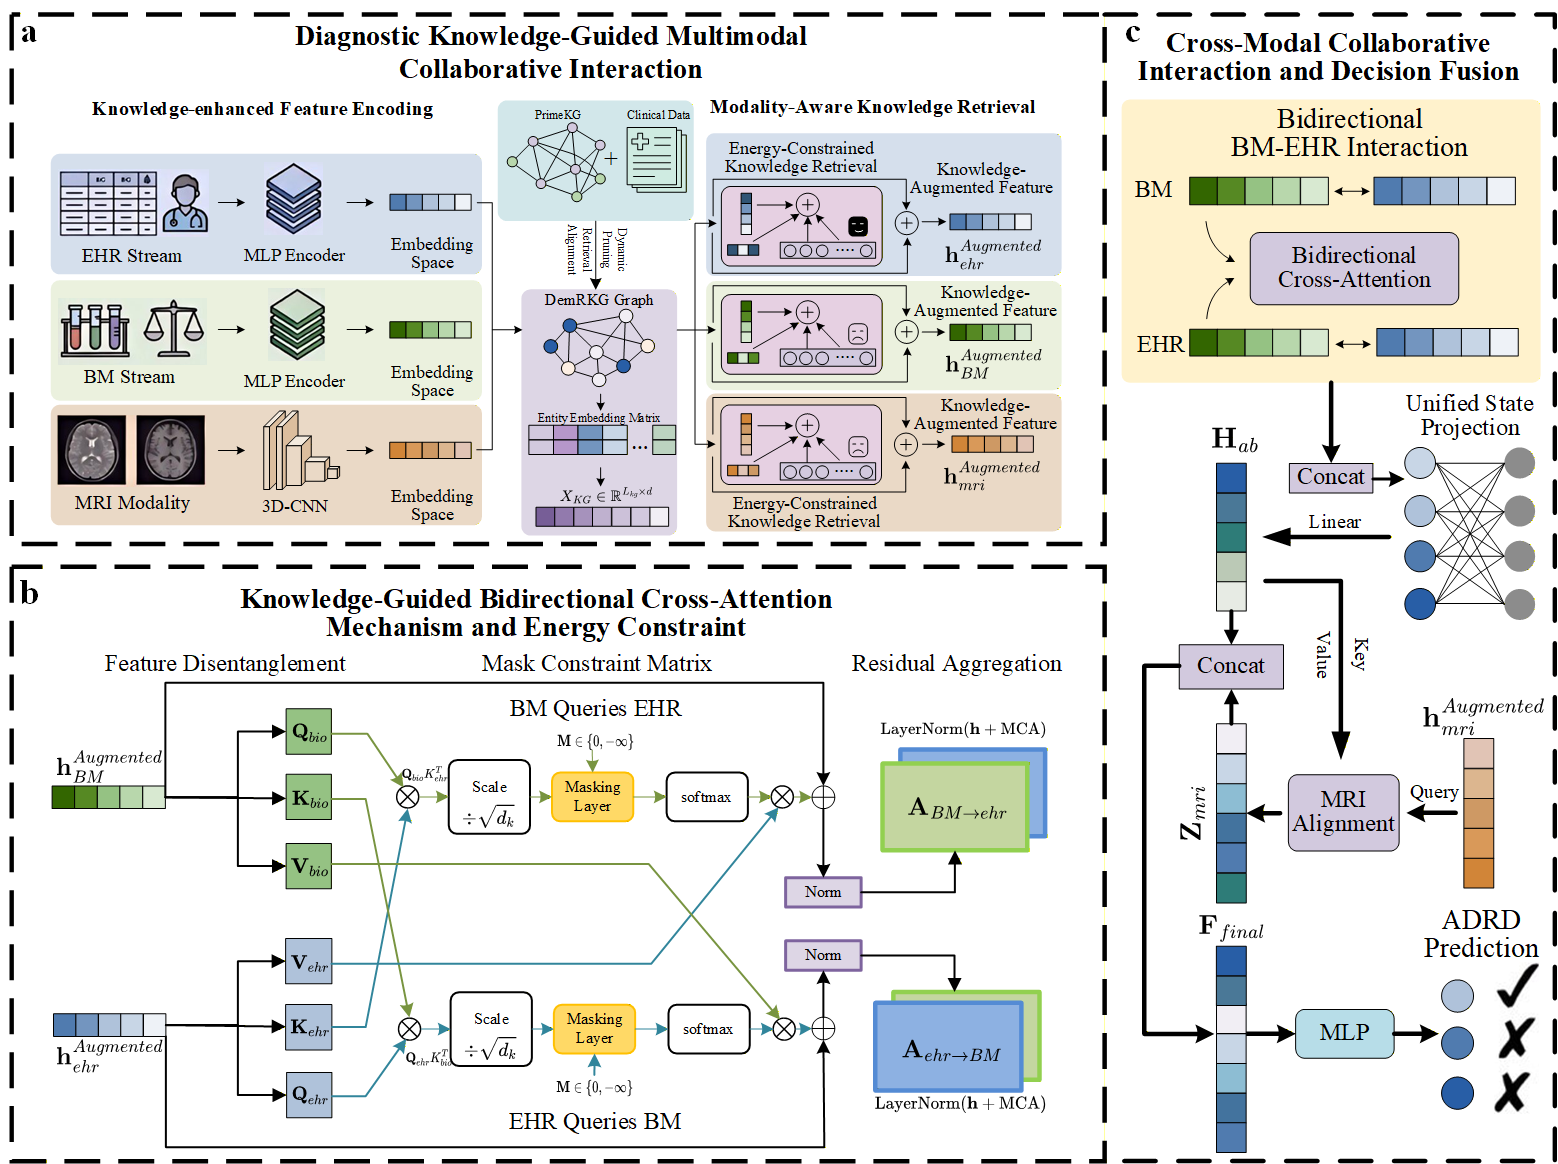
\includegraphics[width=\textwidth]{Figures/KAMT-Trans框架图.png}
        \caption{Overall architecture of KAMT. (a) Knowledge-Augmented encoding and modality-aware retrieval from KG sub-graphs. (b) Masked cross-attention for knowledge injection and the proposed energy-constrained refinement. (c) BM-EHR collaboration guides MRI alignment; the final prediction is made from the fused low-level state and aligned MRI representation.}
        \label{fig:KAMT_framework}
    \end{figure*}

    %\textcolor{purple}{Roles and functions of energy-constrained refinement pathway are still unclear.}
    \textcolor{blue}{The three branches query the same patient knowledge sequence through branch-specific adapters and attention mappings. The conditional free energy below determines the knowledge weights for each branch.}

\subsubsection{\textcolor{blue}{Conditional free energy and knowledge weighting}}

    \textcolor{blue}{For patient $i$ and branch $m\in\{\mathrm{EHR},\mathrm{BM},\mathrm{MRI}\}$, a learned projection of $\mathbf h_{im}$ gives the Query. The DemRKG embeddings pass through the branch-specific adapter $A_m$ before separate learned projections produce the Keys and Values. For a single attention head:}
    \begin{equation}
        {\color{blue}
        \begin{aligned}
        g_{imj}&=A_m(\mathbf X_{KG}^{(i)}[j]),\\
        q_{im}&=W_m^Q\mathbf h_{im}+b_m^Q,\\
        k_{imj}&=W_m^Kg_{imj}+b_m^K,\\
        v_{imj}&=W_m^Vg_{imj}+b_m^V.
        \end{aligned}
        }
        \label{eq:knowledge_qkv}
    \end{equation}

    \textcolor{blue}{On the nonempty patient support $J_i$, the feasible weights lie in $\Delta(J_i)=\{\alpha\in\mathbb R_+^{L_{kg}}:\sum_j\alpha_j=1,\ \alpha_j=0\ (j\notin J_i)\}$. The reference $u_i(j)=1/|J_i|$ is uniform over this support. We define the compatibility energy as $\epsilon_{imj}=-q_{im}^{\mathsf T}k_{imj}/\sqrt{d_k}$, where $d_k$ is the Key dimension per head. The knowledge weights minimize the conditional free energy:}
    \begin{equation}
        {\color{blue}
        \boxed{
        \begin{aligned}
        \alpha_{im}^{*}&=\arg\min_{\alpha\in\Delta(J_i)}\mathcal F_{im}(\alpha),\\
        \mathcal F_{im}(\alpha)&=-\sum_{j\in J_i}\alpha_j
        \frac{q_{im}^{\mathsf T}k_{imj}}{\sqrt{d_k}}\\
        &\quad+D_{\mathrm{KL}}(\alpha\Vert u_i).
        \end{aligned}
        }
        }
        \label{eq:energy_min}
    \end{equation}

    \textcolor{blue}{The energy term favors entities compatible with the current modality representation. Deviations from the uniform reference over $J_i$ are penalized by the KL term. DemRKG's relation-trained embeddings enter the energy through the Keys; patient activation determines the valid positions over which the weights are distributed.}

    \textcolor{blue}{For fixed Queries and Keys, the unique minimizer is}
    \begin{equation}
        {\color{blue}
        \begin{aligned}
        \alpha_{imj}^{*}&=
        \begin{cases}
        \displaystyle\frac{e^{-\epsilon_{imj}}}
        {\sum_{\ell\in J_i}e^{-\epsilon_{im\ell}}},&j\in J_i,\\[6pt]
        0,&j\notin J_i,
        \end{cases}\\
        \mathcal F_{im}(\alpha)-\mathcal F_{im}(\alpha^*)
        &=D_{\mathrm{KL}}(\alpha\Vert\alpha^*)\geq0.
        \end{aligned}
        }
        \label{eq:knowledge_optimum}
    \end{equation}
    \textcolor{blue}{Substituting the energy definition gives masked softmax:}
    \begin{equation}
        {\color{blue}
        \alpha_{im}^*=\operatorname{softmax}
        \left(\frac{K_{im}^{\mathsf T}q_{im}}{\sqrt{d_k}}+M_i\right),
        }
        \label{eq:knowledge_weights}
    \end{equation}
    \textcolor{blue}{where $K_{im}=[k_{im1},\ldots,k_{imL_{kg}}]$, and $M_i(j)=0$ for $j\in J_i$ or $-\infty$ otherwise. The weights $\alpha_{im}^*$ then control Value readout.}

\subsubsection{\textcolor{blue}{Knowledge readout and residual update}}

    \textcolor{blue}{Given the optimal weights $\alpha_{im}^{(a)*}$ from \cref{eq:knowledge_weights}, each of the $H$ attention heads aggregates the corresponding Values over the nonempty support $J_i$ of patient $i$. The head outputs are concatenated and projected to obtain the knowledge response:}

    \begin{equation}
        {\color{blue}
        \begin{aligned}
        \mathbf{z}_{im}^{kg}&=W_m^O\operatorname{Concat}_{a=1}^{H}\left(
        \sum_{j\in J_i}\operatorname{DropAttn}
        (\alpha_{im}^{(a)*})_j v_{imj}^{(a)}\right)\\
        &\quad+b_m^O,
        \end{aligned}
        }
        \label{eq:knowledge_response}
    \end{equation}

    \textcolor{blue}{where $\operatorname{DropAttn}$ applies attention-weight dropout during training and is the identity at inference; $W_m^O,b_m^O$ are the output projection parameters. The optimality in \cref{eq:knowledge_optimum} applies to the weights before this dropout.}
    \textcolor{blue}{When $J_i=\varnothing$, each head instead reads the first zero-input placeholder, whose attention weight is 1 before dropout.}

    Clinical knowledge \textcolor{blue}{is integrated by residual addition and layer normalization}:
    \begin{equation}
    \mathbf{h}_{\textcolor{blue}{i}m}^{Augmented} = \mathrm{LayerNorm}(\mathbf{h}_{\textcolor{blue}{i}m} + \mathbf{z}_{\textcolor{blue}{i}m}^{kg})
    \end{equation}

\subsubsection{\textcolor{blue}{Multimodal fusion and classification}}

    \textcolor{blue}{The augmented BM and EHR features interact through bidirectional cross-attention, with learned projections supplying the Queries, Keys, and Values. Their directional outputs are concatenated and passed through $P_{ab}$, a mapping comprising Linear, ReLU, and Dropout layers, to obtain the joint clinical representation $\mathbf{H}_{ab}$:}

    \begin{equation}
        \begin{aligned}
        \mathbf{A}_{BM \rightarrow ehr}
        &= \mathrm{LayerNorm}\bigl(\mathbf{h}_{BM}^{Augmented}\\
        &\qquad + \mathrm{MCA}(\mathbf{Q}_{BM}, \mathbf{K}_{ehr}, \mathbf{V}_{ehr})\bigr), \\
        \mathbf{A}_{ehr \rightarrow BM}
        &= \mathrm{LayerNorm}\bigl(\mathbf{h}_{ehr}^{Augmented}\\
        &\qquad + \mathrm{MCA}(\mathbf{Q}_{ehr}, \mathbf{K}_{BM}, \mathbf{V}_{BM})\bigr).
        \end{aligned}
        \label{eq:bidirectional_mca}
    \end{equation}

    \begin{equation}
        \mathbf{H}_{ab} = \textcolor{blue}{P_{ab}}\Big(\big[\mathrm{Squeeze}(\mathbf{A}_{BM \rightarrow ehr}) \parallel \mathrm{Squeeze}(\mathbf{A}_{ehr \rightarrow BM})\big]\Big).
        \label{eq:hab_def}
    \end{equation}


    The augmented MRI features \textcolor{blue}{are projected to the Query for cross-attention with $\mathbf{H}_{ab}$ as the Key and Value inputs. For classification, $\mathbf{H}_{ab}$ is concatenated with the resulting MRI representation $\mathbf{Z}_{mri}$ to form $\mathbf{F}_{final}$:}

    \begin{equation}
        \mathbf{Z}_{mri} = \mathrm{LayerNorm}(\mathbf{h}_{mri}^{Augmented} + \mathrm{MCA}(\mathbf{Q}_{mri}, \mathbf{H}_{ab}, \mathbf{H}_{ab})).
        \label{eq:mri_alignment}
    \end{equation}

    \begin{equation}
    \mathbf{F}_{final} = [ \mathrm{Squeeze}(\mathbf{H}_{ab}) \parallel \mathrm{Squeeze}(\mathbf{Z}_{mri}) ].
    \label{eq:final_fusion}
    \end{equation}

    \textcolor{blue}{An MLP classifier produces logits $z_{i,c}$ from $\mathbf{F}_{final}$. Softmax gives the class probabilities, from which the $C$-class cross-entropy loss is computed over a batch of size $B$:}

    \begin{equation}
        \hat{y}_{i,c} = \frac{\exp(z_{i,c})}{\sum_{j=1}^{C} \exp(z_{i,j})}
        \label{eq:softmax}
    \end{equation}

    \begin{equation}
        \mathcal{L}_{CE} = - \frac{1}{B} \sum_{i=1}^{B} \sum_{c=1}^{C} y_{i,c} \log(\hat{y}_{i,c})
        \label{eq:cross_entropy}
    \end{equation}

    where $y_{i,c}$ is the one-hot ground-truth label. \textcolor{blue}{Adding $L_2$ regularization on the learnable parameters $\theta$ gives the training objective:}

    \begin{equation}
        \mathcal{L}_{KAMT} = \mathcal{L}_{CE} + \lambda \sum_{w \in \theta} w^2
        \label{eq:total_loss}
    \end{equation}

    \textcolor{blue}{where $\lambda$ is the regularization coefficient. We optimize \cref{eq:total_loss} using Adam \cite{kingma2014adam}. The conditional free energy in \cref{eq:energy_min} determines $\alpha^*$ during each forward pass; these weights affect classification through Value readout, residual updates, and multimodal fusion.}

\section{Experimental outcomes and analysis}


\subsection{Dataset Descriptions}
% TODO(method-audit, 2026-10-17): 红色比例待核：分类 notebook 的约 64/16/20 与下文常模构建的 70/10/20 尚未统一。
This study used four different datasets: ADNI\cite{weiner2013adni}, NACC\cite{beekly2007nacc}, AIBL\cite{ellis2009aibl}, and PPMI\cite{marek2011ppmi}. The first three datasets focus on Alzheimer's disease (AD), recording clinical observations of normal controls (NC), patients with mild cognitive impairment (MCI), and AD patients, respectively. Meanwhile, the PPMI dataset tracks four disease stages of Parkinson's disease (PD), including its prodromal phase. All datasets are first divided into an initial training set and a clean test set in an \textcolor{red}{8:2 ratio}. Then, the initial training set is divided into a final training set and a validation set in an \textcolor{red}{8:2 ratio}. The sample distribution and scale statistics of the datasets are summarized in \cref{tab:dataset_statistics}.


\begin{table}[htbp]
    \centering
    \caption{Statistics and Description of the Evaluated Datasets}
    \label{tab:dataset_statistics}
    \begin{tabular}{llccc}
        \toprule
        \textbf{Dataset} & \textbf{Task} & \textbf{Class} & \textbf{Count} & \textbf{Total} \\
        \midrule
        \multirow{3}{*}{ADNI} & \multirow{3}{*}{3-Class} & NC & 211 & \multirow{3}{*}{837} \\
        & & MCI & 475 & \\
        & & AD & 151 & \\
        \midrule
        \multirow{3}{*}{NACC} & \multirow{3}{*}{3-Class} & NC & 2,116 & \multirow{3}{*}{3,708} \\
        & & MCI & 879 & \\
        & & AD & 713 & \\
        \midrule
        \multirow{3}{*}{AIBL} & \multirow{3}{*}{3-Class} & NC & 358 & \multirow{3}{*}{516} \\
        & & MCI & 86 & \\
        & & AD & 72 & \\
        \midrule
        \multirow{4}{*}{PPMI} & \multirow{4}{*}{4-Class} & Control & 125 & \multirow{4}{*}{409} \\
        & & PD & 132 & \\
        & & SWEDD & 72 & \\
        & & Prodromal & 80 & \\
        \bottomrule
    \end{tabular}
\end{table}

\subsection{Knowledge Extraction and Graph Visualization}
\subsubsection{Knowledge Representation Extraction}

Taking the NACC dataset as an example, the construction process of DemRKG is as follows: First, 61 clinical and demographic features of the cohort are compared with specific biomedical entities in PrimeKG. Clinical assessments, such as the Boston Naming Test and Connectivity Test A, are directly mapped to phenotypic nodes such as "aphasia" and "executive dysfunction." These targets are activated by comparing them with a global blacklist of irrelevant domains (e.g., drug exposure and off-label use). Then, we retrieve the direct one-hop neighborhoods of these seed nodes, retaining 17,666 medical edges after cleaning. Subsequent two-hop graph traversal utilizes topological relevance to truncate the first 5 nodes, introducing 28,742 high-quality expansion edges. The final DemRKG backbone contains 6,547 entities across 17 relation types, totaling 42,909 triples.

Patient data integration follows a dynamic mapping workflow based on demographic standardization. The training, test, and validation sets were partitioned in a \textcolor{red}{7:2:1 ratio}. Baseline metrics were stratified by age and education level within the normal control (NC) group of the training set to establish standard population norms. Specific nodes in the input sequence were activated only when clinical scores deviated from their corresponding norms by more than 1.5 standard deviations. For behavioral metrics and medical history, activation was triggered when the absolute threshold was greater than zero; the threshold for the Geriatric Depression Scale (GDS) was set to 5 or higher. The maximum length of each patient sequence was 45. Ultimately, this workflow mapped 3383 out of 3708 NACC individuals, generating 30335 valid feature maps for the downstream multimodal architecture.

\subsubsection{Graph Scale Statistics}
The statistics of the knowledge graphs associated with each dataset are presented in Table~\ref{tab:kg_statistics}. As shown in the table, the unrefined original external knowledge base, PrimeKG, exhibits a massive expansion in graph scale. Across all diagnostic cases, PrimeKG introduces a wide range of fundamental biomedical entities (primarily covering a massive number of gene, protein, anatomical structure, and disease nodes). The total number of PrimeKG nodes related to all cases remains above 50,000, and the number of triplets ranges from 3.7 million to 6.0 million. Such an unfiltered and massive structure is highly likely to cause "semantic overload," which interferes with the cross-attention mechanism of KAMT by introducing noise from peripheral nodes.

The graph scale of the private knowledge, CustomKG, shows a strict positive correlation with the number of clinical feature records and the sample size of the datasets. The CustomKG network is mainly composed of patient nodes and feature nodes reflecting demographics, clinical history, and cognitive scale tests. Taking the NACC cohort, which has the most abundant data records, as an example, thousands of patient nodes derive more than 290,000 triplets. In contrast, limited by a smaller sample size or missing clinical records, the scales of CustomKG for the AIBL and PPMI datasets are much smaller.

DemRKG highlights excellent knowledge completion and constraint capabilities. Building upon CustomKG, DemRKG precisely retains microscopic nodes highly related to the disease, such as genes, proteins, and biological processes. For example, in the AIBL dataset, after the construction of DemRKG, the network expanded from a mere 44 clinical feature nodes to 3,894 nodes. This demonstrates that the rich heterogeneity of DemRKG can fill the gaps in the underlying medical logic, establishing a reliable connection between macroscopic symptoms and microscopic molecules.
\begin{table}[!t]
\centering
\caption{Knowledge Graph Scale Statistics}
\label{tab:kg_statistics}
\setlength{\tabcolsep}{8pt}
\renewcommand{\arraystretch}{1.15}
\begin{tabular}{c c r r}
\hline
\textbf{Dataset} & \textbf{Graph Type} & \textbf{Entities} & \textbf{Triplets (Edges)} \\
\hline
\multirow{3}{*}{ADNI} & CustomKG & 1,103  & 38,106 \\
                    & DemRKG   & 4,099  & 23,630 \\
                    & PrimeKG  & 52,532 & 3,743,954 \\
\hline
\multirow{3}{*}{AIBL} & CustomKG & 560    & 3,612 \\
                    & DemRKG   & 3,894  & 22,621 \\
                    & PrimeKG  & 50,061 & 3,712,962 \\
\hline
\multirow{3}{*}{NACC} & CustomKG & 4,003  & 291,673 \\
                    & DemRKG   & 6,547  & 42,909 \\
                    & PrimeKG  & 65,728 & 6,033,272 \\
\hline
\multirow{3}{*}{PPMI} & CustomKG & 677    & 16,410 \\
                    & DemRKG   & 2,497  & 13,050 \\
                    & PrimeKG  & 53,195 & 4,230,076 \\
\hline
\end{tabular}
\end{table}

\subsubsection{DemRKG Visualization}
To intuitively demonstrate the topological morphology of the refined graph, this section takes the DemRKG of the NACC dataset as an example, as shown in \cref{fig:dementia_viz}.

\begin{figure}[!t]
    \centering
    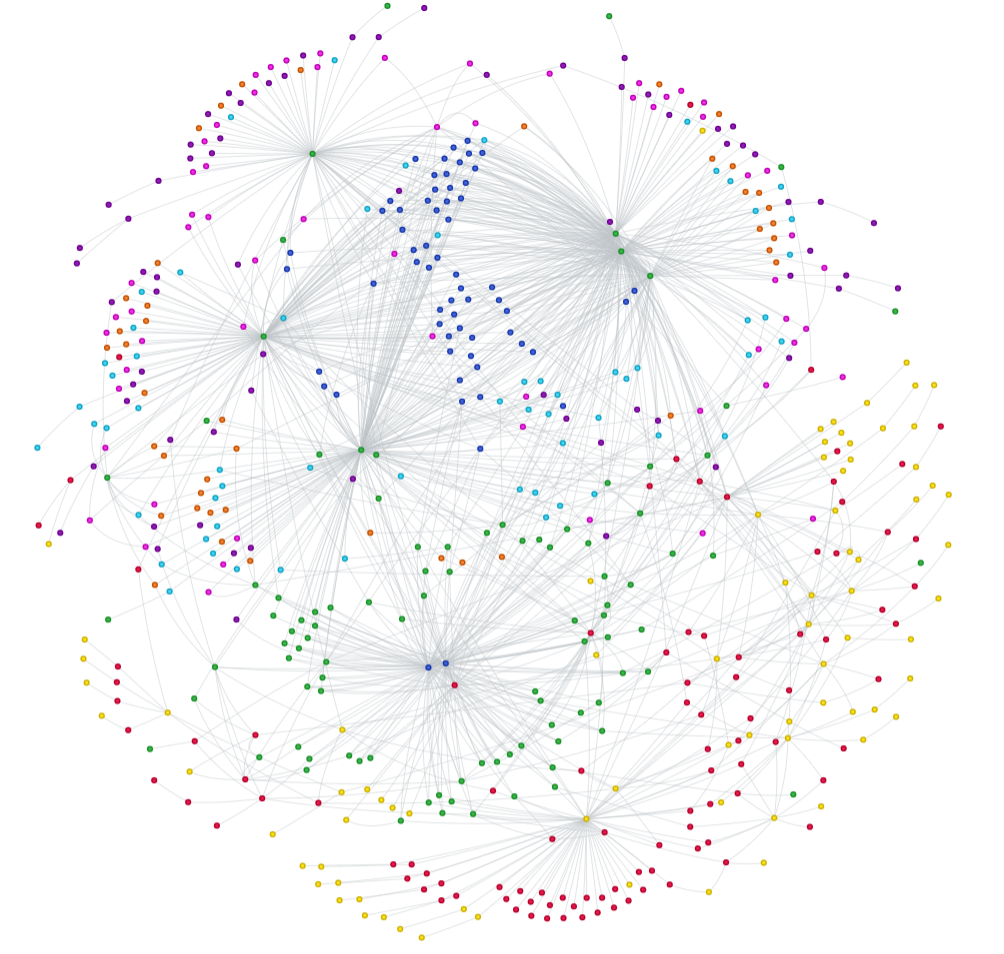
\includegraphics[width=0.85\linewidth]{Figures/NACC-DementiaHKG.png}
    \caption{Visualization of the NACC DemRKG: Integrating multi-dimensional microscopic entities such as genes, proteins, and diseases.}
    \label{fig:dementia_viz}
\end{figure}

Observing the generated visualization, the DemRKG in \cref{fig:dementia_viz} presents itself as a multi-dimensional semantic network. Nodes of different colors form multiple tightly connected local clusters, and the graph incorporates independent entities representing genes, proteins, cellular components, and even molecular functions. Distinct from the divergent planar networks composed of single clinical phenotypes, this highly heterogeneous, interwoven state of nodes intuitively reflects the deep integration of external medical knowledge with private patient data. This structure builds a bridge between macroscopic clinical symptoms and microscopic protein abnormalities, elevating the upper limit of the graph's semantic representation capacity.




\subsection{Performance Comparison}

\begin{table*}[htbp]
\centering
\caption{Performance comparison of different methods on the AIBL, ADNI, NACC, and PPMI datasets}
\label{tab:performance_comparison}
\renewcommand{\arraystretch}{1.3} % 调整行高，使表格不显得拥挤
\begin{tabular}{llccccc}
\toprule
\textbf{Dataset} & \textbf{Method} & \textbf{Accuracy} & \textbf{Precision} & \textbf{Recall} & \textbf{F1 Score} & \textbf{AUC-ROC} \\
\midrule
\multirow{6}{*}{AIBL} 
& MM-Trans (Bi-modal)  & 0.5402 $\pm$ 0.0423 & 0.3704 $\pm$ 0.0542 & 0.3725 $\pm$ 0.0458 & 0.3592 $\pm$ 0.0489 & 0.6173 $\pm$ 0.0312 \\
& MM-Trans (Tri-modal) & 0.4816 $\pm$ 0.0311 & 0.4806 $\pm$ 0.0416 & 0.4474 $\pm$ 0.0384 & 0.4146 $\pm$ 0.0603 & 0.4916 $\pm$ 0.0245 \\
& KGT (TransE)         & 0.6843 $\pm$ 0.0387 & 0.5283 $\pm$ 0.1378 & 0.4524 $\pm$ 0.0416 & 0.4419 $\pm$ 0.0305 & 0.7046 $\pm$ 0.0366 \\
& KAMT (CustomKG)      & 0.7783 $\pm$ 0.0138 & 0.6686 $\pm$ 0.0254 & 0.5839 $\pm$ 0.0706 & 0.5898 $\pm$ 0.0545 & 0.8091 $\pm$ 0.0181 \\
& KAMT (PrimeKG)       & 0.8193 $\pm$ 0.0148 & 0.6586 $\pm$ 0.0165 & 0.6597 $\pm$ 0.0177 & 0.6476 $\pm$ 0.0090 & 0.8455 $\pm$ 0.0077 \\
& \textbf{KAMT (DemRKG)} & \textbf{0.8289 $\pm$ 0.0101} & \textbf{0.6977 $\pm$ 0.0253} & \textbf{0.6912 $\pm$ 0.0253} & \textbf{0.6772 $\pm$ 0.0229} & \textbf{0.8660 $\pm$ 0.0259} \\
\midrule
\multirow{6}{*}{ADNI} 
& MM-Trans (Bi-modal)  & 0.5210 $\pm$ 0.0991 & 0.4242 $\pm$ 0.1345 & 0.4139 $\pm$ 0.0543 & 0.3779 $\pm$ 0.0880 & 0.5626 $\pm$ 0.0506 \\
& MM-Trans (Tri-modal) & 0.5770 $\pm$ 0.0526 & 0.5709 $\pm$ 0.0760 & 0.5351 $\pm$ 0.0441 & 0.5232 $\pm$ 0.0392 & 0.7493 $\pm$ 0.0163 \\
& KGT (TransE)         & 0.6298 $\pm$ 0.0632 & 0.6011 $\pm$ 0.0848 & 0.5633 $\pm$ 0.0734 & 0.5650 $\pm$ 0.0815 & 0.7696 $\pm$ 0.0620 \\
& KAMT (CustomKG)      & 0.7239 $\pm$ 0.0315 & 0.5318 $\pm$ 0.1213 & 0.6284 $\pm$ 0.1018 & 0.5735 $\pm$ 0.1092 & 0.8957 $\pm$ 0.0245 \\
& KAMT (PrimeKG)       & 0.7671 $\pm$ 0.0254 & 0.7652 $\pm$ 0.0594 & 0.7095 $\pm$ 0.0768 & 0.6941 $\pm$ 0.0835 & 0.9283 $\pm$ 0.0059 \\
& \textbf{KAMT (DemRKG)} & \textbf{0.8299 $\pm$ 0.0112} & \textbf{0.8183 $\pm$ 0.0045} & \textbf{0.8023 $\pm$ 0.0232} & \textbf{0.8085 $\pm$ 0.0143} & \textbf{0.9456 $\pm$ 0.0069} \\
\midrule
\multirow{6}{*}{NACC} 
& MM-Trans (Bi-modal)  & 0.5638 $\pm$ 0.0061 & 0.2474 $\pm$ 0.0558 & 0.3364 $\pm$ 0.0046 & 0.2591 $\pm$ 0.0153 & 0.5695 $\pm$ 0.0111 \\
& MM-Trans (Tri-modal) & 0.6540 $\pm$ 0.0041 & 0.5470 $\pm$ 0.0129 & 0.5285 $\pm$ 0.0084 & 0.4962 $\pm$ 0.0080 & 0.7020 $\pm$ 0.0034 \\
& KGT (TransE)         & 0.7360 $\pm$ 0.0022 & 0.6574 $\pm$ 0.0148 & 0.6387 $\pm$ 0.0068 & 0.6302 $\pm$ 0.0221 & 0.8242 $\pm$ 0.0031 \\
& KAMT (CustomKG)      & 0.7875 $\pm$ 0.0095 & 0.7439 $\pm$ 0.0094 & 0.7154 $\pm$ 0.0183 & 0.7227 $\pm$ 0.0170 & 0.9128 $\pm$ 0.0030 \\
& \textbf{KAMT (DemRKG)} & \textbf{0.8067 $\pm$ 0.0102} & \textbf{0.7674 $\pm$ 0.0126} & \textbf{0.7395 $\pm$ 0.0180} & \textbf{0.7486 $\pm$ 0.0150} & \textbf{0.9274 $\pm$ 0.0042} \\
\midrule
\multirow{6}{*}{PPMI} 
& MM-Trans (Bi-modal)  & 0.3227 $\pm$ 0.0564 & 0.1501 $\pm$ 0.0485 & 0.2551 $\pm$ 0.0418 & 0.1812 $\pm$ 0.0457 & 0.5345 $\pm$ 0.0222 \\
& MM-Trans (Tri-modal) & 0.4212 $\pm$ 0.0581 & 0.2653 $\pm$ 0.0494 & 0.3647 $\pm$ 0.0631 & 0.2651 $\pm$ 0.0709 & 0.6740 $\pm$ 0.0827 \\
& KGT (TransE)         & 0.3446 $\pm$ 0.0637 & 0.3575 $\pm$ 0.0869 & 0.3264 $\pm$ 0.0493 & 0.3007 $\pm$ 0.0553 & 0.5842 $\pm$ 0.0631 \\
& KAMT (CustomKG)      & 0.4892 $\pm$ 0.0768 & 0.4883 $\pm$ 0.1659 & 0.4379 $\pm$ 0.0722 & 0.4025 $\pm$ 0.0765 & 0.7033 $\pm$ 0.0628 \\
& KAMT (PrimeKG)       & 0.5877 $\pm$ 0.0329 & 0.4738 $\pm$ 0.0959 & 0.5002 $\pm$ 0.0394 & 0.4522 $\pm$ 0.0559 & 0.8285 $\pm$ 0.0156 \\
& \textbf{KAMT (DemRKG)} & \textbf{0.6185 $\pm$ 0.0125} & \textbf{0.6084 $\pm$ 0.0621} & \textbf{0.5462 $\pm$ 0.0084} & \textbf{0.5166 $\pm$ 0.0182} & \textbf{0.8308 $\pm$ 0.0075} \\
\bottomrule
\end{tabular}
\end{table*}

\begin{figure}[!t]
  \centering
  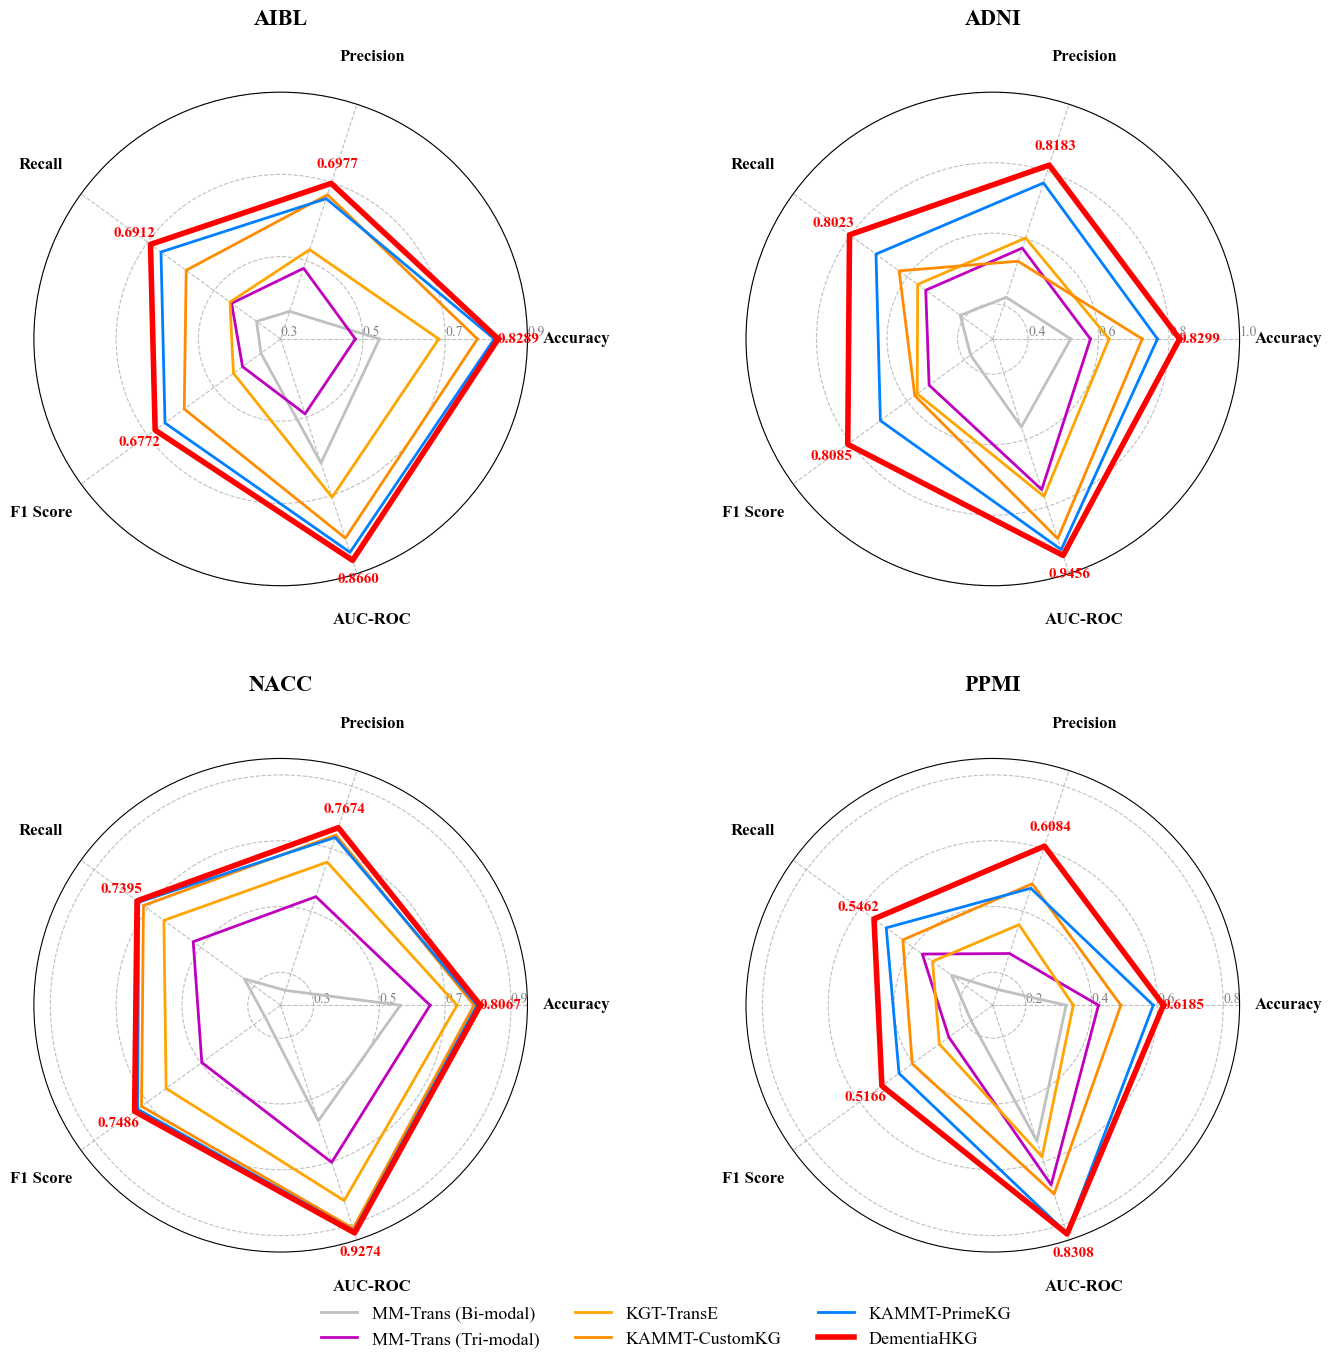
\includegraphics[width=\linewidth]{Figures/雷达图-EN.png}
  \caption{Visual comparison of diagnostic performance across various methods.}
  \label{fig:radar_chart}
\end{figure}

As presented in \cref{tab:performance_comparison} and \cref{fig:radar_chart}, the integration of diverse knowledge representations triggers distinct evolutionary stages in model performance，all metrics are averages obtained from 5-fold cross-validation on the test set. For instance, on the NACC dataset, which features the richest text modality, KGT (TransE) achieves an increase of 0.1340 in F1 Score and 0.0820 in Accuracy compared to the pure data-driven baseline (MM-Trans Tri-modal). However, this upward trend is completely reversed on the PPMI dataset. Facing a complex four-class classification task focused on motor neurodegeneration, KGT (TransE) experiences a noticeable performance degradation, with its accuracy dropping sharply from 0.4212 to 0.3446.

To overcome this performance bottleneck, KAMT (CustomKG) employs DistMult for graph representation learning, which effectively restores and elevates the predictive metrics. In the AIBL dataset, KAMT (CustomKG) increases the Accuracy to 0.7783 (an improvement of 0.0940 over KGT-TransE) and elevates the F1 Score to 0.5898. Furthermore, its AUC-ROC reaches 0.9128 on the NACC dataset. Even under the significant data-missing challenges of the PPMI dataset, the Accuracy successfully recovers to 0.4892.

Building upon these iterative improvements, the proposed KAMT (DemRKG) framework consistently achieves the optimal diagnostic performance across all benchmarks. As intuitively illustrated by the outermost red polygon in \cref{fig:radar_chart}, this approach comprehensively envelops the other baselines. Compared with the standard tri-modal fusion network, incorporating the specialized relational knowledge graph leads to a substantial leap in evaluation metrics. Specifically, the F1 Score of KAMT (DemRKG) improves by approximately 0.285 and 0.262 on the ADNI and AIBL datasets, respectively. Most notably, the Accuracy on the highly challenging PPMI dataset realizes a remarkable surge of nearly 0.20, confirming the robustness of the proposed state-of-the-art solution.
    
Evaluation metrics obtained by the proposed KAMT method demonstrate that our proposed method significantly outperforms traditional baselines and SOTA models.

\textbf{1. Universal Improvement in Training Stability:}
A critical observation across selected benchmarks is the stark contrast in training dynamics. As visualized in our training curves (e.g., Loss and AUC), baseline models (Bimodal/Trimodal without KG) frequently exhibited oscillatory loss patterns and failed to reach optimal convergence, likely due to the non-convex nature of the sparse multimodal feature space. In contrast, the introduction of KG embeddings (DistMult/\textcolor{blue}{DemRKG}) acted as a stabilizer, enabling rapid and smooth convergence in all tasks. This suggests that structured knowledge is not merely an auxiliary feature but a necessary condition for effective optimization in small-sample medical contexts.

\textbf{2. Overcoming the Limitations of Shallow Fusion:}
Traditional data-driven networks inherently rely on crude feature concatenation, which fails to capture complex non-linear interactions. This deficiency is particularly evident in the challenging PPMI dataset, where the Bimodal baseline yields an accuracy of only 0.3227. Our method improves this to 0.6185 by addressing the fundamental semantic gap between different modalities. Instead of merely stacking demographic information (EHR) and clinical scales like UPDRS (Bio) into isolated vector spaces, the KAMT architecture leverages structured knowledge to establish precise decision boundaries, ensuring that discrete clinical signals are firmly anchored to underlying pathological pathways.

\textbf{3. Mitigating Negative Transfer via Bilinear Relational Scoring:}
The severe performance drop of KGT (TransE) on the PPMI dataset exposes the vulnerability of simple translation-based assumptions when modeling complex neurodegenerative diseases. TransE struggles to handle intricate entity relations, consequently introducing noise that corrupts the original multimodal distribution. By utilizing the DistMult scoring function, our framework successfully avoids this negative transfer. The bilinear formulation more efficiently captures latent semantic interactions and similarities among medical entities, producing high-quality, low-redundancy feature representations essential for complex multi-class diagnoses.

\textbf{4. Dynamic Regularization via Knowledge-Aware Cross-Attention:}
Unlike standard architectures that force information compression and obscure critical clinical signals, KAMT allows for fine-grained interaction between precise clinical indicators and external medical knowledge. The cross-attention module within our architecture incorporates a specific mask operation layer. This mask acts as an implicit constraint, utilizing the refined DemRKG to apply dynamic regularization. By strictly defining the "pathological boundaries" for the multimodal learning process, this mechanism dramatically enhances both the overall accuracy and the predictive consistency of the diagnostic model.






\subsection{Ablation Study}
This section disaggregates the specific contributions of knowledge graphs derived from different sources and construction methods to the overall multimodal diagnostic performance.

\subsubsection{Ablation on Knowledge Fusion Mechanisms and Strategies}
To understand the impact of different knowledge graphs within the KAMT architecture, we compare the core metrics of three configurations across various clinical cases: private domain knowledge guidance (CustomKG), an unrefined external knowledge base (PrimeKG), and our proposed relational graph (DemRKG). The comprehensive evaluation is presented in Table \ref{tab:comprehensive_performance}.

\begin{table*}[htbp]
\centering
\caption{Comprehensive performance comparison of diagnostic models}
\label{tab:comprehensive_performance}
\renewcommand{\arraystretch}{1.3} % 调整行高
\begin{tabular}{llccccc}
\toprule
\textbf{Dataset} & \textbf{Method} & \textbf{Accuracy} & \textbf{Precision} & \textbf{Recall} & \textbf{F1 Score} & \textbf{AUC-ROC} \\
\midrule
\multirow{3}{*}{AIBL} 
& KAMT (CustomKG)      & 0.7783 $\pm$ 0.0138 & 0.6686 $\pm$ 0.0254 & 0.5839 $\pm$ 0.0706 & 0.5898 $\pm$ 0.0545 & 0.8091 $\pm$ 0.0181 \\
& KAMT (PrimeKG)       & 0.8193 $\pm$ 0.0148 & 0.6586 $\pm$ 0.0165 & 0.6597 $\pm$ 0.0177 & 0.6476 $\pm$ 0.0090 & 0.8455 $\pm$ 0.0077 \\
& \textbf{KAMT (DemRKG)} & \textbf{0.8289 $\pm$ 0.0101} & \textbf{0.6977 $\pm$ 0.0253} & \textbf{0.6912 $\pm$ 0.0253} & \textbf{0.6772 $\pm$ 0.0229} & \textbf{0.8660 $\pm$ 0.0259} \\
\midrule
\multirow{3}{*}{ADNI} 
& KAMT (CustomKG)      & 0.7239 $\pm$ 0.0315 & 0.5318 $\pm$ 0.1213 & 0.6284 $\pm$ 0.1018 & 0.5735 $\pm$ 0.1092 & 0.8957 $\pm$ 0.0245 \\
& KAMT (PrimeKG)       & 0.7671 $\pm$ 0.0254 & 0.7652 $\pm$ 0.0594 & 0.7095 $\pm$ 0.0768 & 0.6941 $\pm$ 0.0835 & 0.9283 $\pm$ 0.0059 \\
& \textbf{KAMT (DemRKG)} & \textbf{0.8299 $\pm$ 0.0112} & \textbf{0.8183 $\pm$ 0.0045} & \textbf{0.8023 $\pm$ 0.0232} & \textbf{0.8085 $\pm$ 0.0143} & \textbf{0.9456 $\pm$ 0.0069} \\
\midrule
\multirow{3}{*}{NACC} 
& KAMT (CustomKG)      & 0.7875 $\pm$ 0.0095 & 0.7439 $\pm$ 0.0094 & 0.7154 $\pm$ 0.0183 & 0.7227 $\pm$ 0.0170 & 0.9128 $\pm$ 0.0030 \\
& KAMT (PrimeKG)       & 0.7970 $\pm$ 0.0087 & 0.7364 $\pm$ 0.0148 & 0.7330 $\pm$ 0.0156 & 0.7372 $\pm$ 0.0163 & 0.9209 $\pm$ 0.0025 \\
& \textbf{KAMT (DemRKG)} & \textbf{0.8067 $\pm$ 0.0102} & \textbf{0.7674 $\pm$ 0.0126} & \textbf{0.7395 $\pm$ 0.0180} & \textbf{0.7486 $\pm$ 0.0150} & \textbf{0.9274 $\pm$ 0.0042} \\
\midrule
\multirow{3}{*}{PPMI} 
& KAMT (CustomKG)      & 0.4892 $\pm$ 0.0768 & 0.4883 $\pm$ 0.1659 & 0.4379 $\pm$ 0.0722 & 0.4025 $\pm$ 0.0765 & 0.7033 $\pm$ 0.0628 \\
& KAMT (PrimeKG)       & 0.5877 $\pm$ 0.0329 & 0.4738 $\pm$ 0.0959 & 0.5002 $\pm$ 0.0394 & 0.4522 $\pm$ 0.0559 & 0.8285 $\pm$ 0.0156 \\
& \textbf{KAMT (DemRKG)} & \textbf{0.6185 $\pm$ 0.0125} & \textbf{0.6084 $\pm$ 0.0621} & \textbf{0.5462 $\pm$ 0.0084} & \textbf{0.5166 $\pm$ 0.0182} & \textbf{0.8308 $\pm$ 0.0075} \\
\bottomrule
\end{tabular}
\end{table*}

This section compares the core metrics of private domain knowledge guidance (CustomKG), external knowledge base (PrimeKG, without refining), and the relational graph (DemRKG) proposed in this paper under the KAMT architecture in various cases.

As shown by \ref{tab:comprehensive_performance}, after introducing external domain knowledge, PrimeKG's prediction performance is generally better than CustomKG. Taking the ADNI dataset as an example, the PrimeKG solution outperforms CustomKG by $0.0432$ and $0.1206$ in Accuracy and F1 Score, respectively; in the NACC dataset with the richest text modalities, PrimeKG also achieves a higher level in comprehensive evaluation metrics such as AUC-ROC (reaching $0.9209$). The external knowledge base covers multi-dimensional medical consensus, including disease targets and gene expression, effectively compensating for the limitations of semantic association in single internal diagnostic records.

In all cases, DemRKG achieved the best metrics. In the most challenging PPMI four-class classification task, DemRKG improved the accuracy and F1 score by 0.0308 and 0.0644, respectively, compared to the PrimeKG solution using a purely external knowledge base. Ablation experiments verified that the refined relational knowledge graph DemRKG can effectively eliminate redundant connections between medical entities and maintain the performance of diagnostic models even in complex cases.

\subsubsection{Validation of Architectural Generalization and Prediction Stability}
To isolate the contribution of our network design from the knowledge graph, we introduce a baseline model, KAMP (Knowledge-Aware Multimodal Perceiver), which relies on a latent variable bottleneck mechanism. Both architectures are evaluated under identical conditions, integrating the domain-specific DemRKG. The comparative performance across multicenter datasets is detailed in Table \ref{tab:arch_compare}.

\begin{table}[htbp]
    \centering
    \caption{Performance comparison across architectures integrating DemRKG}
    \label{tab:arch_compare}
    \setlength{\tabcolsep}{3.5pt} 
    \resizebox{\linewidth}{!}{%
    \begin{tabular}{llccccc}
        \toprule
        \textbf{Dataset} & \textbf{Backbone} & \textbf{Accuracy} & \textbf{Precision} & \textbf{Recall} & \textbf{F1 Score} & \textbf{AUC-ROC} \\
        \midrule
        \multirow{2}{*}{AIBL} 
        & KAMT & \textbf{0.8289 $\pm$ 0.0101} & \textbf{0.6977 $\pm$ 0.0253} & \textbf{0.6912 $\pm$ 0.0253} & 0.6772 $\pm$ 0.0229 & 0.8660 $\pm$ 0.0259 \\
        \cline{2-7}
        & KAMP   & 0.8193 $\pm$ 0.0108 & 0.6899 $\pm$ 0.0232 & 0.6890 $\pm$ 0.0218 & \textbf{0.6804 $\pm$ 0.0188} & \textbf{0.8689 $\pm$ 0.0079} \\
        \midrule
        \multirow{2}{*}{ADNI} 
        & KAMT & \textbf{0.8299 $\pm$ 0.0112} & \textbf{0.8183 $\pm$ 0.0045} & 0.8023 $\pm$ 0.0232 & \textbf{0.8085 $\pm$ 0.0143} & 0.9456 $\pm$ 0.0069 \\
        \cline{2-7}
        & KAMP   & 0.8254 $\pm$ 0.0060 & 0.8148 $\pm$ 0.0138 & \textbf{0.8038 $\pm$ 0.0186} & 0.8063 $\pm$ 0.0055 & \textbf{0.9477 $\pm$ 0.0033} \\
        \midrule
        \multirow{2}{*}{NACC} 
        & KAMT & \textbf{0.8067 $\pm$ 0.0102} & \textbf{0.7674 $\pm$ 0.0126} & \textbf{0.7395 $\pm$ 0.0180} & \textbf{0.7486 $\pm$ 0.0150} & \textbf{0.9274 $\pm$ 0.0042} \\
        \cline{2-7}
        & KAMP   & 0.7815 $\pm$ 0.0064 & 0.7345 $\pm$ 0.0106 & 0.7071 $\pm$ 0.0133 & 0.7162 $\pm$ 0.0133 & 0.9113 $\pm$ 0.0028 \\
        \midrule
        \multirow{2}{*}{PPMI} 
        & KAMT & \textbf{0.6185 $\pm$ 0.0125} & \textbf{0.6084 $\pm$ 0.0621} & \textbf{0.5462 $\pm$ 0.0084} & \textbf{0.5166 $\pm$ 0.0182} & \textbf{0.8308 $\pm$ 0.0075} \\
        \cline{2-7}
        & KAMP   & 0.5661 $\pm$ 0.0265 & 0.5222 $\pm$ 0.0448 & 0.4962 $\pm$ 0.0269 & 0.4736 $\pm$ 0.0261 & 0.8018 $\pm$ 0.0189 \\
        \bottomrule
    \end{tabular}}
\end{table}

In datasets characterized by a lower density of textual modalities, both architectures exhibit comparable diagnostic capabilities. As demonstrated in Table \ref{tab:arch_compare}, their metrics are nearly equivalent on the AIBL and ADNI datasets. Notably, the KAMP architecture achieves a slightly higher AUC-ROC of 0.9477 on ADNI compared to KAMT's 0.9456. This observation suggests that when the embedding dimensions of text modalities are relatively low, both models can adequately fit the clinical representations and yield reliable predictions.

However, the architectural superiority of KAMT becomes pronounced when handling highly heterogeneous, high-dimensional phenotypic data. In the NACC dataset, which contains the most extensive text modalities, and the Parkinson's disease-specific PPMI dataset, KAMT consistently outperforms the baseline. In the most challenging PPMI classification scenario, KAMT exceeds KAMP by 0.0524 in Accuracy and 0.0430 in F1 Score. This performance gap is directly attributable to the handling of information bottlenecks. KAMP forces complex fine-grained features into a compressed low-dimensional latent space, which inevitably degrades data fidelity. Conversely, KAMT employs a modality-aware strategy that preserves the original distribution of the underlying clinical data, preventing critical signal loss.

\subsubsection{Discussion on the Multimodal Diagnostic Paradigm}
The comprehensive ablation studies systematically validate the efficacy of the "diagnostic knowledge graph guidance combined with multi-omics data" paradigm for complex brain disease diagnosis. The core mechanisms driving this performance improvement can be condensed into three key aspects:

\begin{itemize}
    \item \textbf{Dynamic Regularization via Relational Graph (DemRKG):} By tailoring the broad biomedical consensus of PrimeKG against private domain datasets, DemRKG achieves a critical balance between knowledge breadth and depth. It acts as a dynamic regularizer, constraining the multimodal learning (MML) process and preventing the noise inherent in unrefined external databases.
    
    \item \textbf{Implicit Constraint via Cross-Attention Synergy:} KAMT abandons the brute-force feature stacking of conventional MML. Through a cross-self-attention module paired with a mask operation layer, DemRKG tokens serve as an implicit constraint, guiding the network to actively discover optimal alignments between general pathological relationships and specific clinical signals.
    
    \item \textbf{High-Fidelity Modality Preservation:} Unlike Perceiver-based architectures (KAMP) that compress inputs into a low-dimensional latent bottleneck, KAMT preserves the original distribution of the data. It enables fine-grained interactions between external knowledge and specific inputs—such as Bio clinical scales, EHR demographics, and 3D-CNN preprocessed MRI features—capturing the subtle pathologies essential for accurate diagnosis.
\end{itemize}







\subsection{Investigation of Clinical Knowledge Representations}

Table \ref{tab:comprehensive_performance} shows that \textcolor{blue}{DemRKG} leads to a secondary leap in performance. Based on the universal convergence improvements observed, we identify the following core mechanisms:

\subsubsection{Stabilization of Optimization Landscape (Global Mechanism)}
    
The primary contribution of the \textcolor{blue}{KGE learning} is its role as a powerful \textbf{Regularizer}. In medical multimodal learning, the feature space is often high-dimensional yet sparse, creating a highly volatile loss landscape. The injection of pre-trained KG embeddings (DistMult/\textcolor{blue}{DemRKG}) provides a stable ``skeleton'' (manifold) for the feature space. This significantly reduces the search space for the Multimodal Transformer, ensuring consistent convergence across all datasets (ADNI, PPMI, NACC), preventing the model from collapsing into random guessing.

\subsubsection{Semantic Anchoring Effect}

Pure data-driven models treat clinical attributes as isolated symbols. By anchoring attributes (e.g., \texttt{upd2315a}) to standardized entities in \textcolor{blue}{DemRKG} (e.g., \texttt{Symptom:Rest\_Tremor}), the model acquires a clear \textbf{Inductive Bias}. This ``God's eye view'' acts as a navigational aid, guiding the gradient descent towards biologically meaningful solutions.

The \textbf{Hierarchical Instantiation Strategy} ($\text{Patient} \to \text{Level} \to \text{Concept}$) bridges the gap between samples. It ensures that patients with varying symptom severities are drawn closer in the embedding space through shared parent concepts, effectively mitigating the overfitting issues common in small-sample medical data.


\section{Discussion}
\subsubsection{Dynamic Regularization and Efficient Structural Representation}

As illustrated in \cref{fig:accuracy_boxplot}, pure data-driven baseline networks (MM-Trans) exhibit significant prediction fluctuations and numerous outliers across four independent cohorts. When facing complex cases with unclear boundaries, these unguided multi-modal alignment processes easily learn spurious shortcuts rather than true pathological patterns. To stabilize the learning process, KAMT introduces the refined DemRKG. Rather than merely appending information, knowledge tokens work with a mask operation layer within the cross-attention module to act as an implicit dynamic constraint. This mechanism establishes strict pathological boundaries for optimizing high-dimensional features, effectively preventing random feature drift in complex spaces and improving overall diagnostic reliability. To process the dense structural knowledge within DemRKG efficiently, the architecture employs the bilinear scoring function of the DistMult algorithm. DistMult captures latent semantic interactions among biological entities and reduces computational redundancy, supplying high-quality structural priors that make the dynamic regularization process both robust and computationally viable.

\begin{figure}[!t]
    \centering
    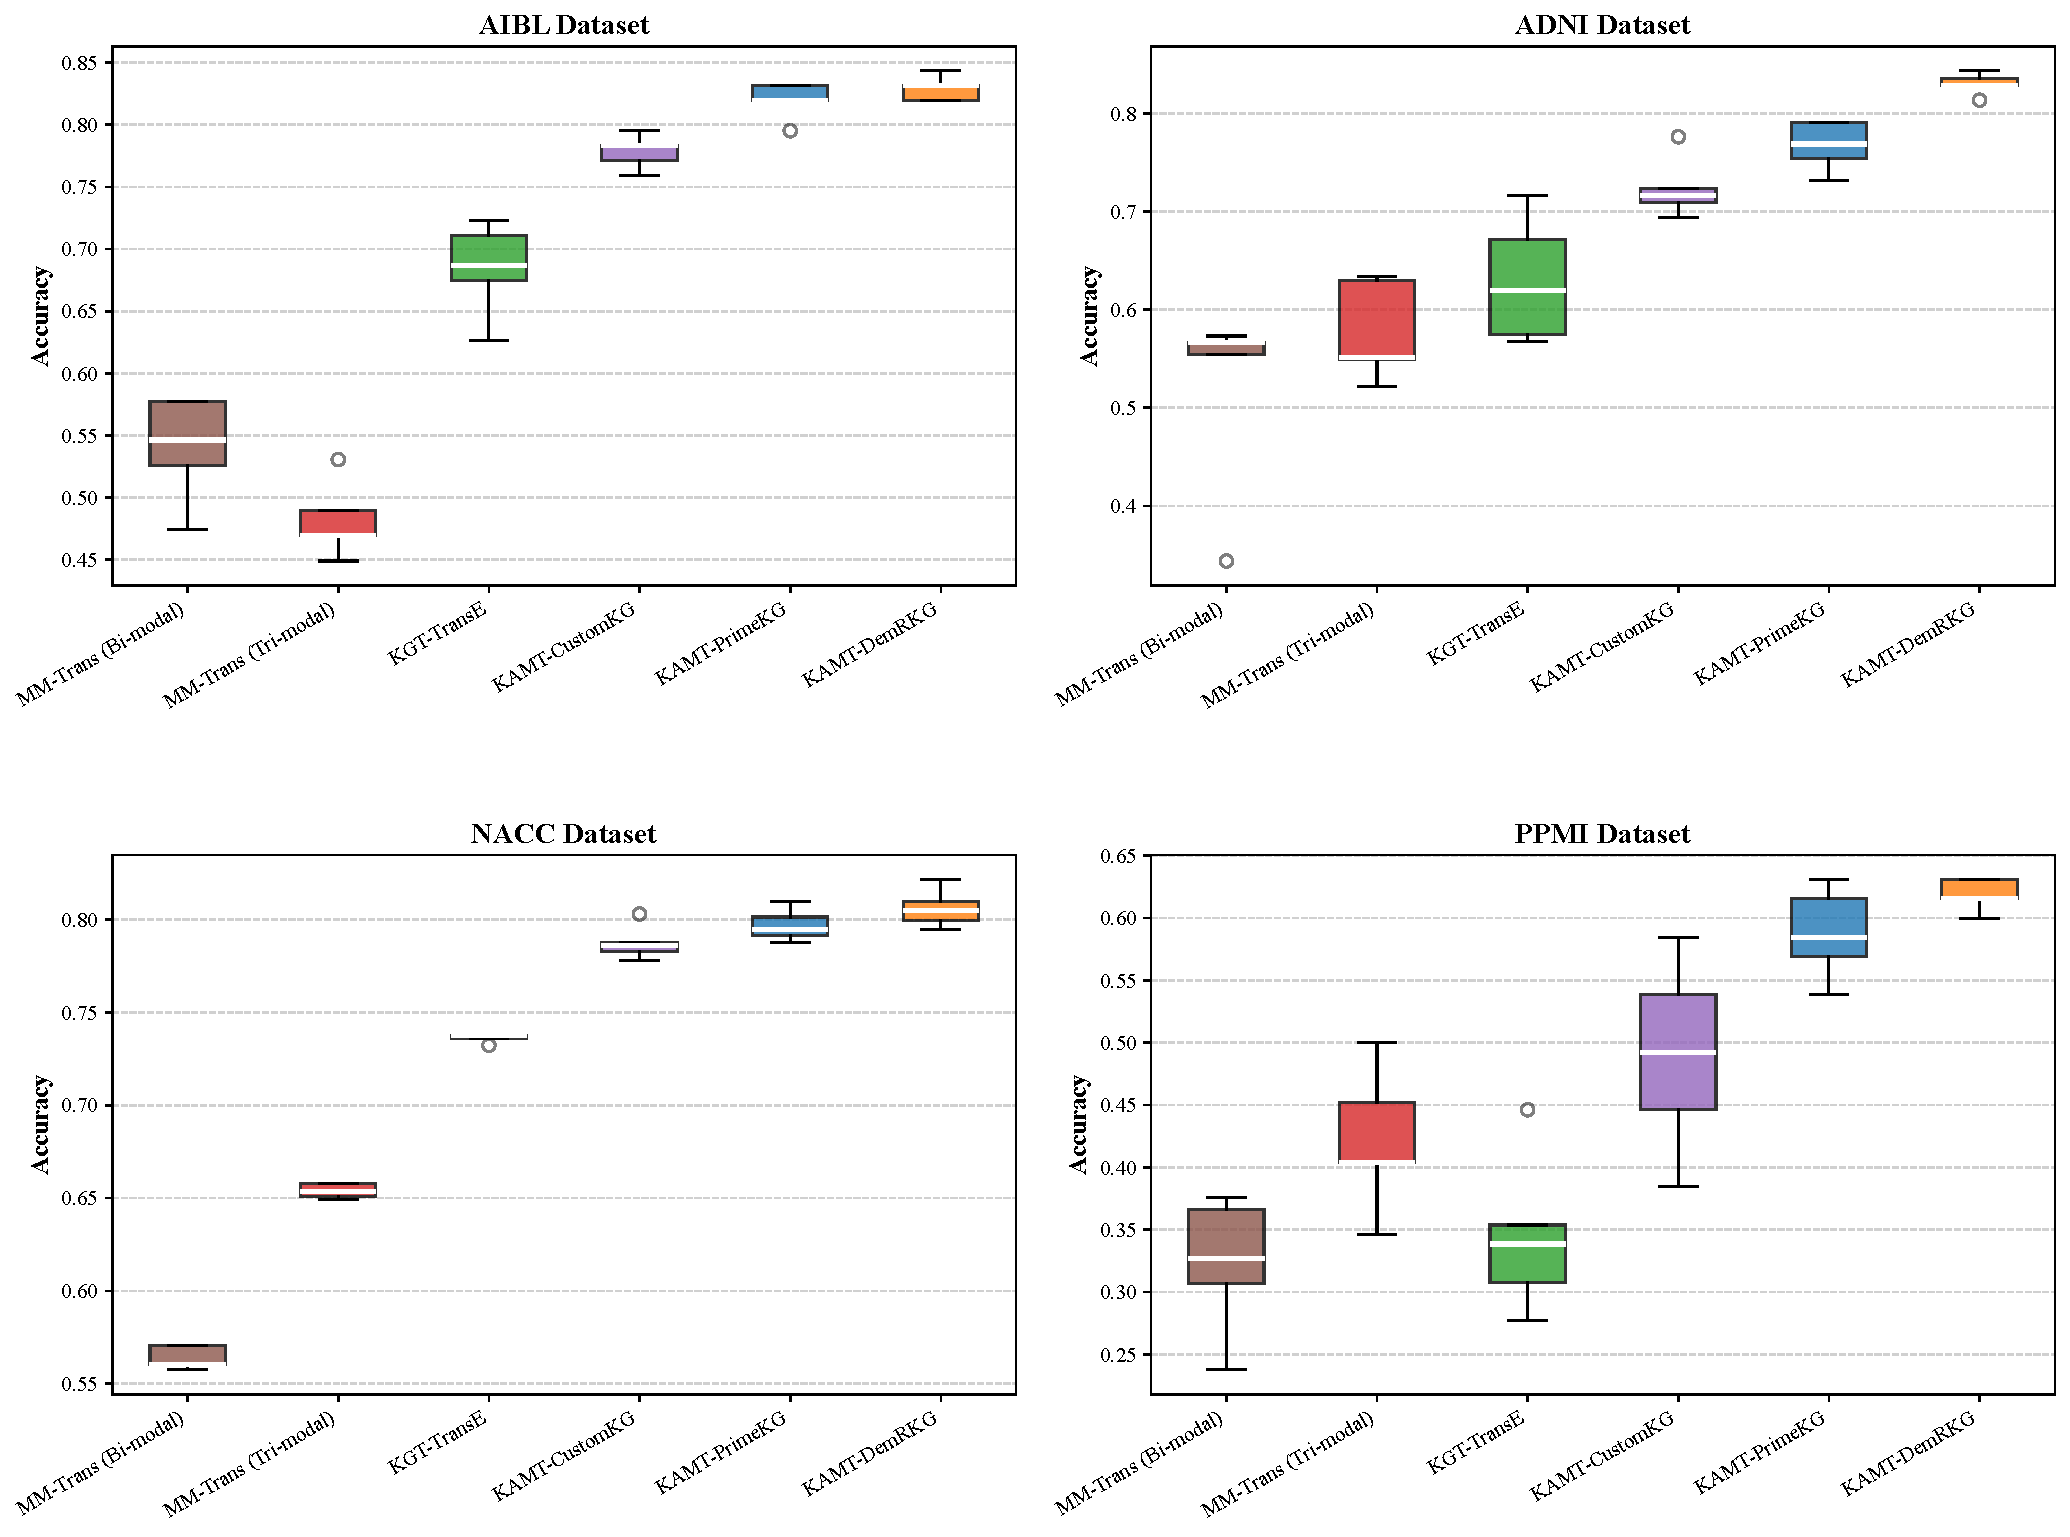
\includegraphics[width=0.9\linewidth]{Figures/箱型图-EN.pdf}
    \caption{Boxplot of prediction accuracy distribution across four independent cohorts.}
    \label{fig:accuracy_boxplot}
\end{figure}

\subsubsection{Semantic Preservation in Fine-Grained Alignment}

Fine-grained diagnostic tasks often suffer from severe performance drops when networks forcefully compress input features. For instance, the Perceiver mechanism in traditional KAMP architectures relies on an information bottleneck that causes irreversible semantic loss. This compression is particularly damaging for dense textual modalities, sweeping away critical details such as basic demographic data in the EHR module and specific clinical scales like UPDRS in the Bio module. To prevent this degradation, the KAMT architecture enforces strict dimensional matching between Queries and Keys. This specific design creates a point-to-point interconnection between clinical observations and DemRKG nodes, ensuring that every clinical scale value aligns perfectly with its corresponding micro-pathological knowledge. Guided by the implicit constraints of the knowledge tokens, the cross-modal features are optimized via energy minimization. Consequently, the network firmly adheres to actual clinical observations without sacrificing the integrity of fine-grained semantic features.


\subsubsection{Clinical Limitations and Real-World Applicability}

Despite its strong cross-center diagnostic efficacy, the real-world clinical deployment of the proposed framework remains constrained by its dependency on complete cross-sectional data snapshots, the loss of complex topological integrity during spatial knowledge representation, and an absence of transparent causal reasoning pathways. To bridge these gaps, future research will focus on integrating missing-modality-aware mechanisms for dynamic longitudinal tracking, leveraging higher-dimensional graph neural networks to preserve edge-level semantic priors, and coupling the architecture with logical path-tracking algorithms to reconstruct interpretable reasoning chains.

%\section{Data availability}

    %\textcolor{blue}{The Parkinson’s Progression Markers Initiative (PPMI, http://www.ppmi-info.org/) database and the Parkinson’s Disease Biomarkers Program (PDBP, https://pdbp.ninds.nih.gov/) database used in this study are both accessible through AMP-PD (https://amp-pd.org/). To access clinical and omics data at the AMP-PD Tier 2 level, users are required to complete a data use agreement and submit an online application.}
	

%\section*{Code availability}

	%This M$^2$STGAT method is implemented in Python and available in Github (https://github.com/ZJ-BMDmining/M2DGAT).


    
%\section*{Acknowledgment}

	%This work is sponsored by National Natural Science Foundation of China(62302455, 62172369), Special Support Plan for High-level Talents in Zhejiang Province(2021R52019) and Natural Science Foundation of Zhejiang Province, China(LQ24F030007).
	
	

%\section*{References}
\bibliographystyle{unsrt}
\bibliography{references.bib}




\vfill

\end{document}


